% !TEX root = main.tex
\section{Systematic uncertainties}
\label{sec:Systematics}


This section covers all relevant systematic uncertainties on the measured observables.
In particular, the model dependent description of the invariant $\Bs$ mass spectrum, the parametrization of the time acceptance using cubic splines, 
as well as the scaling of the time resolution and tagging calibration are potential sources of systematic errors. 
The largest contribution of systematic uncertainty is expected to appear in the choice of amplitudes entering the model to describe the 5 dimensional phase space, discussed in Section \ref{sec:fullFit}.

\subsection{Models for $\Bs$ mass distribution}
\label{subsec:SystMass}

The statistical subtraction of the residual background \cite{Pivk:2004ty}, left after the full selection, relies on the correct description of the invariant $\Bs$ mass distribution.
Since the choice of signal and background models is not unique, alternative descriptions which lead to slightly different yields for the signal and background components are available. 
The difference in yields could result in shifted values for the measured observables and are therefore treated as systematic uncertainty. \newline

\subsubsection{Signal model}

The Johnson's SU function which is used as nominal signal model is replaced by a double Crystal Ball \cite{CB}. 
The crystal ball model is given by a gaussian core with an exponential tail on one side. 
Choosing a double Crystal Ball allows for asymmetric tails in a slightly different way compared to the Johnson's SU function. 
%Table xXx summarizes the observed differences in signal and background yields.

\subsubsection{Background model}

For the description of the partially reconstructed background, 
a combination of the RooHILLdini and RooHORNsdini model \cite{Hill:2253246} is used instead of the nominal model of three bifurcated gaussians. 
The HORNSdini model is used to describe the $\Bs\to\Ds^{*}[\to\Ds(\piz)] X_{s/d}$ decay, where the brackets around the $\piz$ indicate that it is missed in the reconstruction. 
The $\Ds^{*}\to\Ds\piz$ decay is a Vector $\to$ Scalar-Scalar ($1^{-}\to 0^{-}0^{-}$) transition. 
Using the helicity of the $\Ds$, one can show that this results in a double-peak structure in the reconstructed $\Bs$ mass. 
Therefore, the HORNSdini shape consists of a gaussian-like double-peak structure:

\begin{equation}
HORNS(m_{\Bs}) = \int^{b}_{a} dm_{\Bs}\left(m_{\Bs} - \frac{a+b}{2} \right)^{2}\mathcal{DG}(m_{\Bs}\vert\mu,\sigma,f_{G})\left(\frac{1-\zeta}{b-a}m_{\Bs} + \frac{b\zeta - a}{b - a} \right),
\label{eq:HORNS}
\end{equation}

where a and b are the kinematic endpoins of the distribution and $\zeta$ is the positive, real fraction of the two peak hights. Additionaly, the shape is convoluted with a gaussian to account for resolution effects.

The HILLdini model parametrizes the invariant mass shape of $\Bs\to\Ds^{*}[\to\Ds(\gamma)] X_{s/d}$ candidates, where the $\gamma$ is not reconstructed.
Contrary to the previously discussed process, the $Ds^{*}\to\Ds\gamma$ is a Vector $\to$ Scalar-Vector ($1^{-} \to 0^{-} 1^{-}$) transition. 
From helicity arguments, the expected shape in the mass distribution of $\Bs$ candidates follows a parabolic curve without any peaking structure.
To accommodate for this shape, the HILLdini model consists of a parabolic curve between the kinematic endpoints a \& b: 


\begin{equation}
HILL(m_{\Bs}) = \begin{cases} -(m_{\Bs} - a)(m_{\Bs} - b),& \mbox{for } a < m_{\Bs} < b \\
 0, &  otherwise. \end{cases}
\label{eq:HILLS}
 \end{equation}

This shape is convoluted with the same gaussian resolution function used for the HORNSdini model.
%The resulting differences in yields is shown in Table xXx. \newline


To study systematic uncertainties originating from the description of the combinatorial background, the nominal second order polynomial is replaced by an exponential function. 
%The changes in signal and background yields after refitting with this alternative shape are shown in Table xXx. \newline

\subsubsection{Description of misidentified background}

The fixed shape and yield of the mis-ID background in the $m(\Ds\kaon\pion\pion)$ spectrum is another source of systematic uncertainty.
To evaluate this possible source arising from the description of the single mis-ID of $\Bs\to\Ds^{(*)}\pion_{\kaon}\pion\pion$ candidates, we vary the yield of this component as follows:

\begin{itemize}
 
\item We fix the yield of the mis-ID components to zero.

\item We double the yield of the mis-ID components.

\item We quadruple the yield of the mis-ID components.

\end{itemize}

For the shape of the mis-ID background, 
the nominal approach is to use a simulated sample of $\Bs\to\Ds^{-}\pip\pim\pip$ or $\Bs\to\Ds^{*-}\pip\pim\pip$ 
decays and flip the mass hypothesis of the $\pip$ with the higher misidentification probability (see Sec. \ref{sec:massFits}). 
The resulting $m(\Ds^{(*)}\pion_{\kaon}\pion\pion)$ distribution is then modelled and the shape obtainted from the fit is used in the nominal mass fit to signal. This approach is modified as follows:

\begin{itemize}

\item We flip the mass hypothesis of the $\pip$ candidate with the lower probability of beeing misidentified. 

\item We randomly flip the mass hypothesis of a $\pip$ candidate.

\end{itemize}

For the five variations of the misidentified background component, new signal sWeights are generated and the time dependent fit is reiterated. 


\subsubsection{Systematic effect on observables}

The shift of the central values of the observables in the full fit when using sWeights obtained from a combination of alternative models, 
as well as using only one alternative model for the signal/comb.background/part.reco.background and keeping the nominal model for the other parts,
is shown in Table \ref{tab:SystSummary}. 
%We conservatively choose the biggest variation as systematic uncertainty from the modelling of the invariant $\Bs$ mass spectrum.



\subsection{Decay-time acceptance}
\label{subsec:SystTime}

To investigate the systematic uncertainty related to the decay-time dependent efficiency, we vary our parametrization of the acceptance using cubic splines.
This is explicitly done by choosing slightly different knot positions, 
varying the spline coefficients at the nominal positions within their statistical uncertainties and adding/subtracting knots in the range $0.4\ps < t < 11\ps$.
Additionaly, an adaptive binning scheme is used to determine the knot positions in a way that roughly equal amounts of data is covered between two knots.
Strictly speaking, the variation of the spline coefficients within their uncertainty gives the statistical uncertainty of the decay-time acceptance parametrization.
For the presented measurement, this is done using the Cholesky decomposition  \cite{Golub:1996:MC:248979} of the covariance matrix of coefficients $c_{i}$, 
generating toy splines with randomized coefficient values $c_{i,toy}$ from this decomposition and refitting using the toy spline.  
Furthermore, the fit to the decay-time distribution of signal $\Bs\to\Ds\pion\pion\pion$ candidates, used to determine the spline parametrization, is reiterated with varying fixed/constrained values for $\DGs$.


\subsubsection{Varition of knot positions}
The nominal knot positions are changed to be:

\[ k_{alt1}(t) =  [0.5\mbox{ } 1 \mbox{ }1.5 \mbox{ }2 \mbox{ }3 \mbox{ }6 \mbox{ }9.5], 
\mbox{ } k_{alt2}(t) =  [0.5 \mbox{ } 1\mbox{ }  1.5 \mbox{ } 2 \mbox{ } 3\mbox{ }  9\mbox{ } 11],  
\mbox{ } k_{adaptive}(t) =  [0.7\mbox{ } 1.2\mbox{ } 1.7\mbox{ } 2.2\mbox{ } 6.3] \]

The variation of knot positions is found to give a neglectable effect when compared to the variation of spline coefficients.

\subsubsection{Variation of spline coefficients}

Due to the sizeable correlation of the spline coefficients $c_{i}$ determined in Chapter \ref{sec:timeAcceptance}, 
the variations of the observables in the amplitude fit when changing one spline coefficient can not be added up in quadrature for all coefficients.
To simplify the problem, a Cholesky decomposition \cite{Golub:1996:MC:248979} is used to generate a set of uncorrelated vectors from the covariance matrix $A_{cov}$.
It can be shown that every Hermitian positive-definite matrix, such as $A_{cov}$, has a unique Cholesky decomposition of the form:

\begin{equation}
A_{cov} = L \cdot L^{T},
\label{eq:choleskyDecomp}
\end{equation}

where $L$ is a lower triangular matrix with real and positive diagonal entries and $L^{T}$ denotes the transpose of $L$. \newline

Given the four free spline coefficients which are determined from the fit described in \ref{sec:Acceptance}, $A_{cov}$ is a $4x4$ matrix. Therefore, the lower triangular matrix $L$ is of the form:

\begin{equation}
L = \begin{pmatrix}
v_{11} & 0 & 0 & 0 \\
v_{12} & v_{22} & 0 & 0 \\
v_{13} & v_{23} & v_{33} & 0\\ 
v_{14} & v_{24} & v_{34} & v_{44}
\end{pmatrix},
\label{eq:choleskyVectors}
\end{equation}


where $v_{ij}$ are real and positive numbers. $L$ contains four row vectors, which are by construction the four decorrelated modes of the covariant matrix $A_{cov}$. 
From this modes, one can form variations for each of the spline coefficients:

\begin{equation}
c_{i} = c_{nom,i} + \Sigma_{j} \left(r_{j} \cdot v_{ij} \right),
\label{eq:choleskyCoeffs}
\end{equation}

where $i=1..4$, $c_{i}$ is the i-th generated coefficient of the toy spline, $c_{nom,i}$ is the i-th coefficient determined from the nominal decay-time dependent fit to $\Bs\to\Ds\pion\pion\pion$, 
$r_{j}$ are normally distributed real random numbers from a distribution of unit width and $v_{ij}$ are the components of $L$ (where $i$ is the row index and $j$ the column index). \newline
We now generate four sets of 100 toy splines, where one of the four spline coefficients is varied each time using Eq. \ref{eq:choleskyCoeffs}. 
Thus, the time-dependent amplitude fit is repeated in total 400 times with a generated toy spline and the shift of the mean value of the physics observables over each of the $4\cdot100$ sets is quoted as 
uncertainty arising from $c_{i=1..4}$. The uncertainties are then added in quadrature to form the overall uncertainty due to the spline coefficients. %Table \ref{table:Pulls_tDFit_noChol} summarizes the results of this study.

%\begin{table}[hp!]
\centering
\caption{Pull parameters for CP coefficients from the toy studies for the time-dependent fit.}
\begin{tabular}{l | c | c}
\hline
Parameter & $\mu$ of pull distribution & $\sigma$ of pull distribution \\
\hline
\hline
C & 0.00271841 $\pm$ 0.00159745 & 0.0694972 $\pm$ 0.00127009 \\
D & -0.0115746 $\pm$ 0.00755454 & 0.331063 $\pm$ 0.00576761 \\
S & -0.00151265 $\pm$ 0.000852967 & 0.0378623 $\pm$ 0.000754181 \\
$\bar{D}$ & -0.0106657 $\pm$ 0.00746365 & 0.327998 $\pm$ 0.00581649 \\
$\bar{S}$ & -0.00152321 $\pm$ 0.000983966 & 0.0437459 $\pm$ 0.000849528 \\
\hline
\end{tabular}
\label{table:Pulls_tDFit_noChol}
\end{table}



\subsection{Decay-time resolution}

To study systematic effects originating from the scaling of the decay-time resolution $\sigma_{t}$, the decay-time distribution of fake $\Bs$ candidates using prompt $\Ds$ is described by single Gaussian function.
The resultions of the single Gaussians in the different bins of the per-event decay-time error can then be used to derive the scaling function in a straightforward way.
Since the distribution of the fake $\Bs$ decay time does not follow a perfect Gaussian distribution, two different approaches which either slightly overestimate or underestimate the decay time error are used:

\begin{itemize}

\item A double Gaussian is fit to the decay-time distributions of fake $\Bs$ candidates, but only the narrow with of the core Gaussian is considered to represent the time resolution in the respective bin. 
This method assumes that the other, broader Gaussian component does not represent the decay-time resolution of the signal $\Bs$ sample. Therefore the resolution is slightly underestimated in this case.

\item A singel Gaussian is fit to the decay-time distributions of fake $\Bs$ candidates in a wide range of $[-3\sigma_{t} : 1.5\sigma_{t}]$. 
Due to the tails of the distribution, which broaden the width of the Gaussian function, this method slightly overestimates the decay-time resolution.   

\end{itemize}

The widths of the single Gaussians from the fits performed with the two methods in bins of the per-event decay-time error is studied and a new resolution scaling function is derived for both cases: \newline

\begin{equation}
\sigma_{eff}^{core-Gauss}(\sigma_t) = \left(4.9  \pm 2.0 \right) \text{fs} + \left( 0.821 \pm 0.050 \right) \sigma_t
\label{eq:ResoSyst1}
\end{equation}

\begin{equation}
\sigma_{eff}^{single-Gauss}(\sigma_t) = \left(8.3  \pm 1.5 \right) \text{fs} + \left( 0.997 \pm 0.037 \right) \sigma_t
\label{eq:ResoSyst2}
\end{equation}

The scaling functions are shown in Fig. \ref{fig:SystscaleFactor} and the systematic uncertainty to the CP-observables is summarized in Table \ref{tab:SystSummary} .


\begin{figure}[h]
\centering
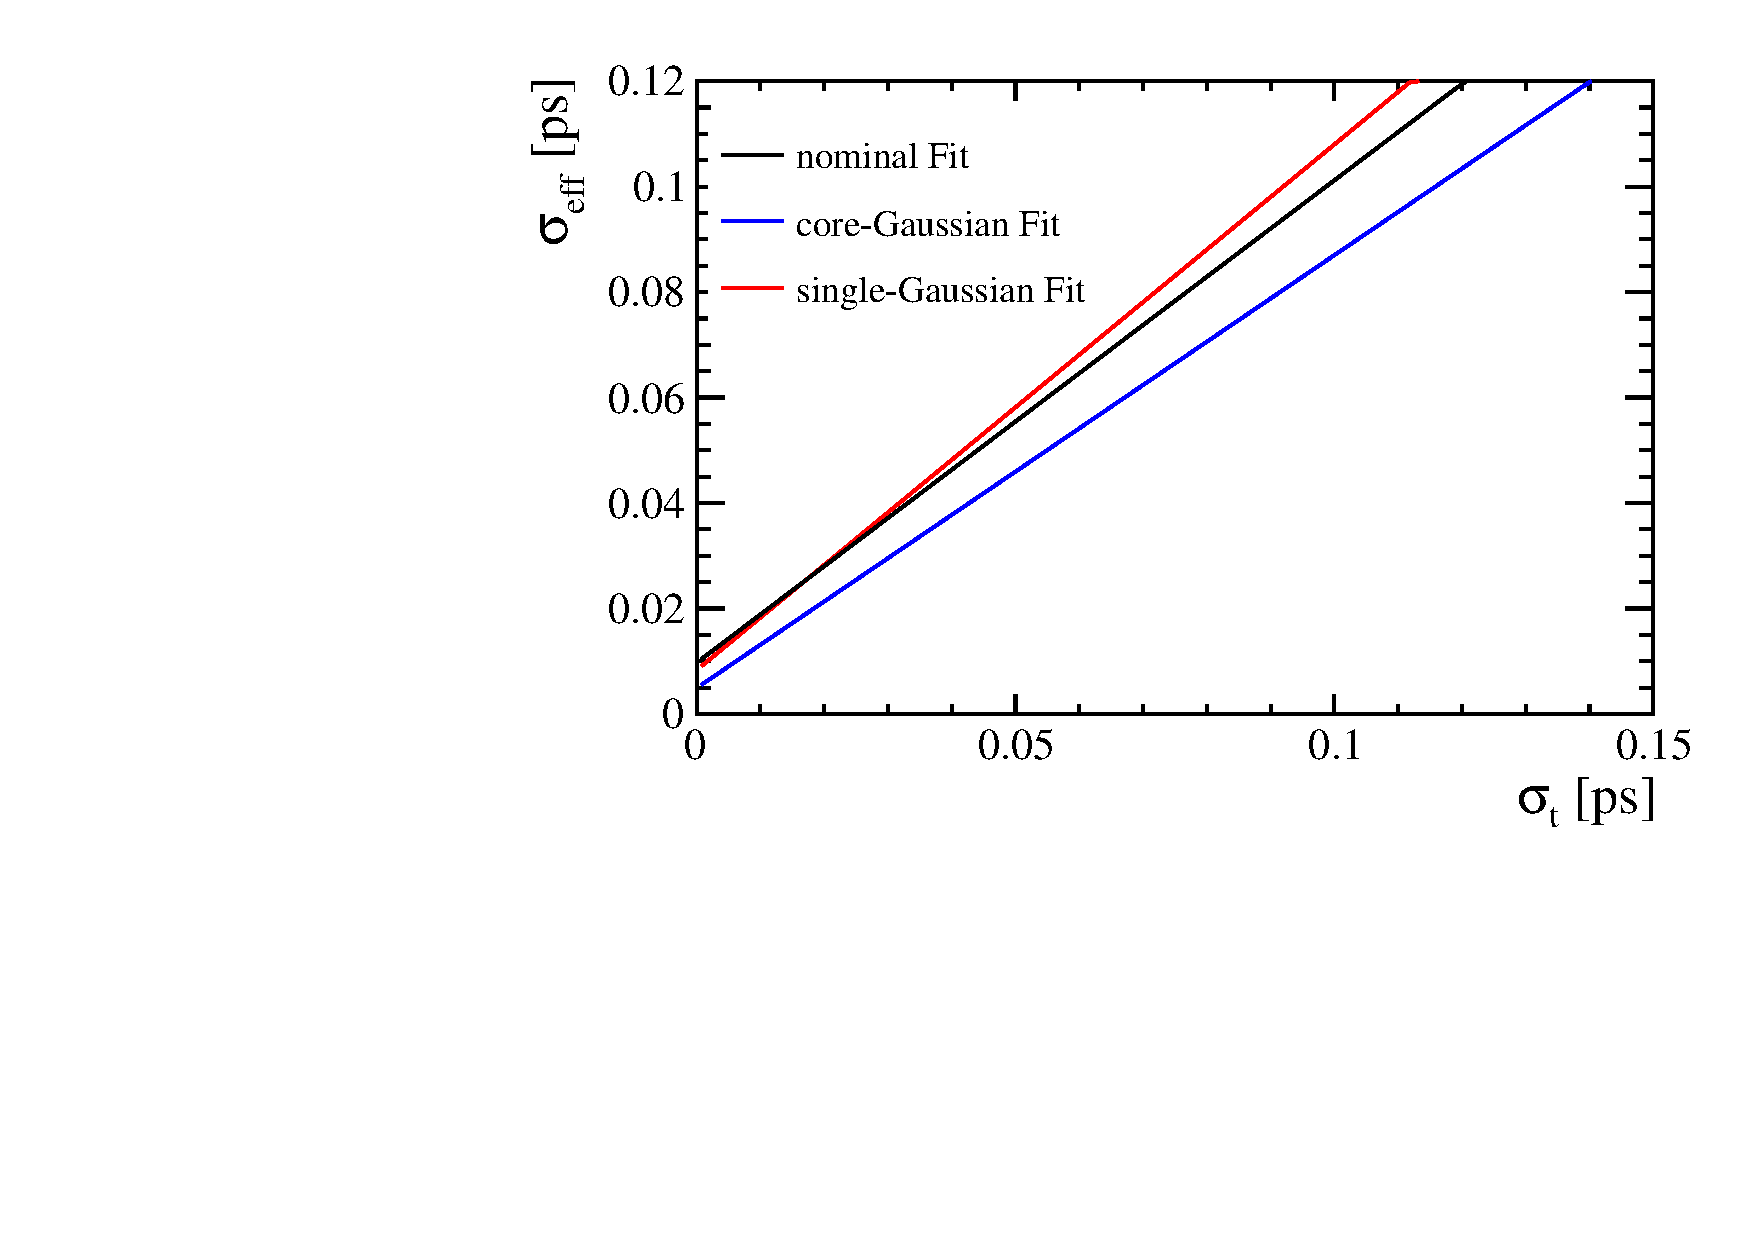
\includegraphics[height=!,width=0.66\textwidth]{figs/Resolution/ResoSyst.pdf}
\caption{The measured resolution scaling function of the per-event decay time error estimate $\sigma_t$ for fake $B_s$ candidates (Run-II data) 
for (black line) the nominal scaling, (blue line) only using the narrow gaussian width of the double gaussian fit model or (red line) when determining the resolution using a single gaussian model.}
\label{fig:SystscaleFactor}
\end{figure}


%\begin{figure}[h]
%\centering
%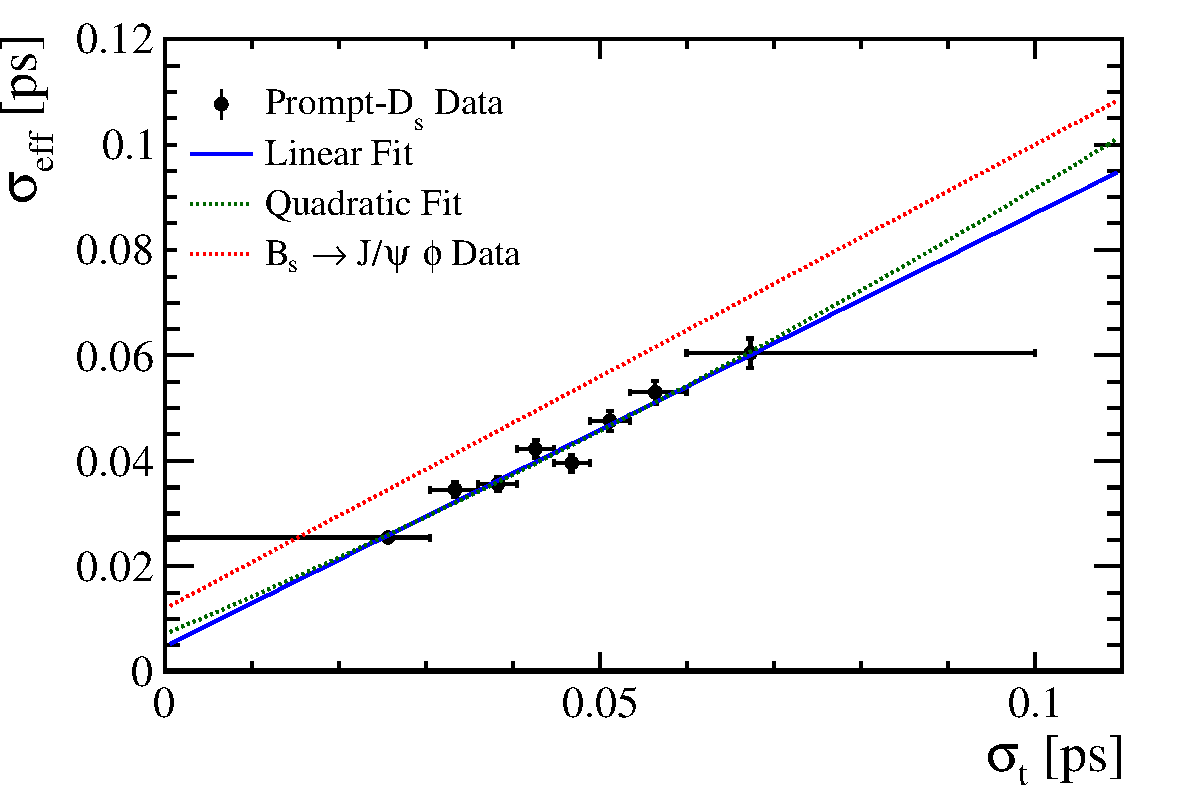
\includegraphics[height=!,width=0.49\textwidth]{figs/Resolution/ScaleFactor_Data_coreGauss.pdf}
%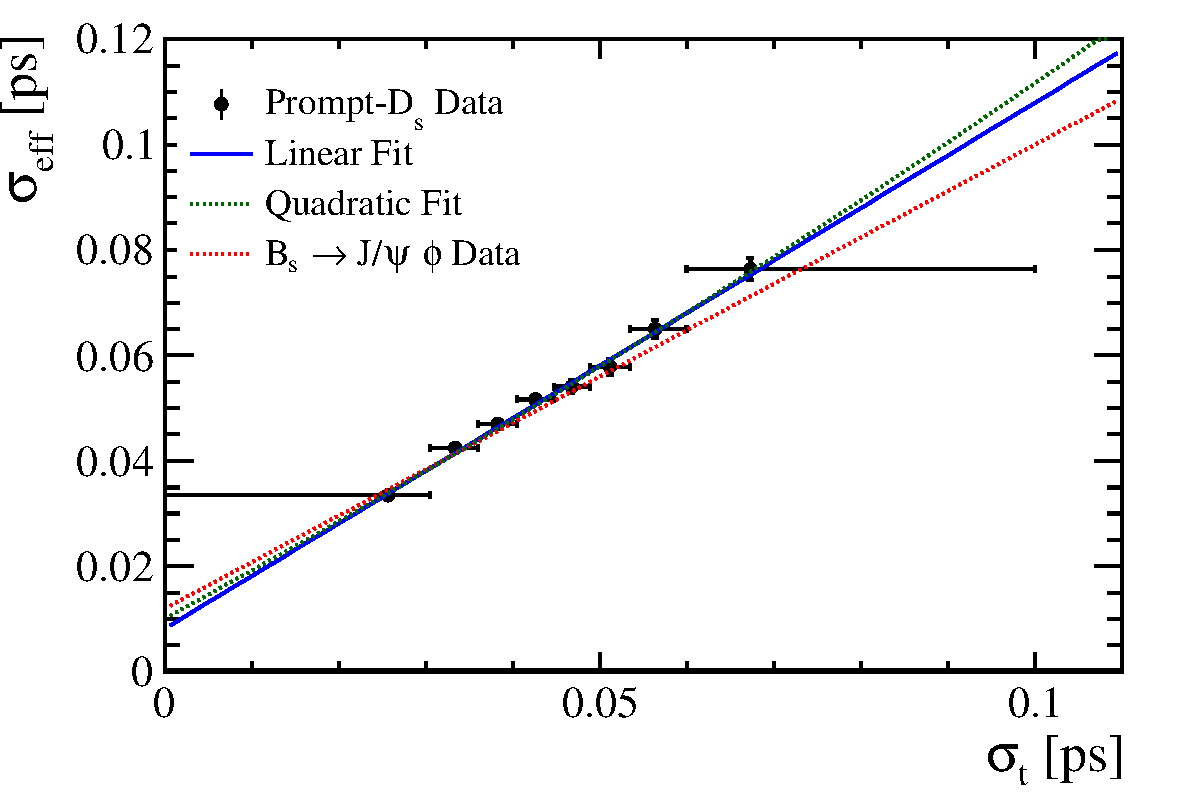
\includegraphics[height=!,width=0.49\textwidth]{figs/Resolution/ScaleFactor_Data_singleGauss.pdf}
%\caption{The measured resolution $\sigma_{eff}$ as function of the per-event decay time error estimate $\sigma_t$ for fake $B_s$ candidates (Run-II data) 
%when (left) only using the narrow gaussian width of the double gaussian fit model or (right) when determining the resolution using a single gaussian model.
%The fitted calibration curve is shown in blue for both cases.}
%\label{fig:SystscaleFactor}
%\end{figure}


\subsection{Tagging calibration}

Systematic uncertainties arise from the statistical precision of the tagging parameters determined from the calibration, discussed in Sec. \ref{sec:Tagging}.
These uncertainties are accounted for by the inclusion of Gaussian constrains in the nominal fit. 
The width of the respective constrain for the tagging parameter $p_{i}$  is chosen to be $\Delta p_{i}$. 
In this way, the systematic uncertainty due to the tagging calibration is included in the statistical uncertainty of the time dependent fit.  

\subsection{Summary of systematic uncertainties}

All contributing systematic uncertainties are summarized in Table \ref{tab:SystSummary}. 
The individual uncertainties are summed in quadrature to arrive at the total systematic uncertainty for the respective CP observable.
Their total magnitude ranges from (30-40)$\%$ of the statistical uncertainty of the fit.


\clearpage

\begin{table}[h]
\centering
\caption{Systematic uncertainties on the fit parameters of the phase-space integrated fit to $B_s \to D_s K\pi \pi$ data in units of statistical standard deviations.}
\resizebox{\linewidth}{!}{
	\renewcommand{\arraystretch}{1.5}
	\begin{tabular}{l  c  c  c  c  c  c  c  c  c  c  c  | c }
\hline
\hline
Fit Parameter & Fit bias & Time-Acc. & Resolution & $\Delta m_{s}$ & Asymmetries & Background & Lineshapes & Resonances $m,\Gamma$ & Form-Factors & Phsp-Acc. & Amp. Model &  Total  \\ 
\hline
$B_s \to D_s \, ( K_1(1270) \to K^{*}(892) \, \pi ) \, \text{Mag}$ & 0.10 & 0.01 & 0.04 & 0.01 & 0.00 & 0.13 & 0.48 & 0.24 & 0.52 & 0.06 &  & 0.77 \\ 
$B_s \to D_s \, ( K_1(1270) \to K^{*}(892) \, \pi ) \, \text{Phase}$ & 0.07 & 0.01 & 0.04 & 0.01 & 0.01 & 0.08 & 0.35 & 0.28 & 0.34 & 0.12 &  & 0.58 \\ 
$B_s \to D_s \, ( K_1(1270) \to K^{*}_{0}(1430) \, \pi ) \, \text{Mag} $ & 0.04 & 0.01 & 0.01 & 0.00 & 0.00 & 0.24 & 1.44 & 0.11 & 0.17 & 0.04 &  & 1.47 \\ 
$B_s \to D_s \, ( K_1(1270) \to K^{*}_{0}(1430) \, \pi ) \, \text{Phase} $ & 0.04 & 0.01 & 0.02 & 0.01 & 0.00 & 0.19 & 5.83 & 0.19 & 0.61 & 0.09 &  & 5.87 \\ 
$B_s \to D_s \, ( K_1(1400) \to K^{*}(892) \, \pi ) \, \text{Mag} (b \to c)$ & 0.13 & 0.03 & 0.16 & 0.06 & 0.02 & 0.34 & 1.32 & 0.37 & 0.78 & 0.19 &  & 1.64 \\ 
$B_s \to D_s \, ( K_1(1400) \to K^{*}(892) \, \pi ) \, \text{Phase} (b \to c)$ & 0.14 & 0.02 & 0.09 & 0.02 & 0.01 & 0.18 & 0.54 & 0.26 & 0.40 & 0.08 &  & 0.77 \\ 
$B_s \to D_s \, ( K_1(1400) \to K^{*}(892) \, \pi ) \, \text{Mag} (b \to u)$ & 0.10 & 0.04 & 0.05 & 0.12 & 0.04 & 0.32 & 0.35 & 0.22 & 0.73 & 0.16 &  & 0.93 \\ 
$B_s \to D_s \, ( K_1(1400) \to K^{*}(892) \, \pi ) \, \text{Phase} (b \to u)$ & 0.02 & 0.04 & 0.04 & 0.10 & 0.03 & 0.08 & 0.79 & 0.21 & 0.31 & 0.08 &  & 0.89 \\ 
$B_s \to D_s \, ( K^{*}(1410) \to K^{*}(892) \, \pi ) \, \text{Mag} (b \to c)$ & 0.08 & 0.03 & 0.08 & 0.08 & 0.03 & 0.18 & 0.61 & 0.25 & 0.75 & 0.28 &  & 1.06 \\ 
$B_s \to D_s \, ( K^{*}(1410) \to K^{*}(892) \, \pi ) \, \text{Phase} (b \to c)$ & 0.35 & 0.01 & 0.06 & 0.01 & 0.01 & 0.13 & 0.60 & 0.19 & 0.68 & 0.08 &  & 1.00 \\ 
$B_s \to D_s \, ( K^{*}(1410) \to K \, \rho(770) ) \, \text{Mag}$ & 0.35 & 0.01 & 0.02 & 0.01 & 0.00 & 0.18 & 0.59 & 0.12 & 0.34 & 0.06 &  & 0.79 \\ 
$B_s \to D_s \, ( K^{*}(1410) \to K \, \rho(770) ) \, \text{Phase}$ & 0.18 & 0.00 & 0.01 & 0.01 & 0.00 & 0.24 & 0.34 & 0.09 & 0.21 & 0.06 &  & 0.51 \\ 
$B_s \to D_s \, ( K(1460) \to K^{*}(892) \, \pi ) \, \text{Mag} (b \to u)$ & 0.14 & 0.03 & 0.05 & 0.05 & 0.02 & 0.37 & 0.43 & 0.27 & 0.60 & 0.12 &  & 0.89 \\ 
$B_s \to D_s \, ( K(1460) \to K^{*}(892) \, \pi ) \, \text{Phase} (b \to u)$ & 0.13 & 0.04 & 0.11 & 0.07 & 0.03 & 0.21 & 0.84 & 0.49 & 0.46 & 0.06 &  & 1.11 \\ 
$B_s \to ( D_s \, \pi)_{P} \, \, K^{*}(892) \, \text{Mag} (b \to c)$ & 0.03 & 0.02 & 0.06 & 0.02 & 0.01 & 0.24 & 0.95 & 0.11 & 0.55 & 0.13 &  & 1.14 \\ 
$B_s \to ( D_s \, \pi)_{P} \, \, K^{*}(892) \, \text{Phase} (b \to c)$ & 0.20 & 0.01 & 0.13 & 0.02 & 0.01 & 0.51 & 1.10 & 0.18 & 0.52 & 0.26 &  & 1.38 \\ 
$B_s \to ( D_s \, \pi)_{P} \, \, K^{*}(892) \, \text{Mag} (b \to u)$ & 0.14 & 0.04 & 0.07 & 0.06 & 0.02 & 0.11 & 0.78 & 0.24 & 0.54 & 0.17 &  & 1.01 \\ 
$B_s \to ( D_s \, \pi)_{P} \, \, K^{*}(892) \, \text{Phase} (b \to u)$ & 0.24 & 0.05 & 0.19 & 0.06 & 0.03 & 0.47 & 1.54 & 0.28 & 0.59 & 0.17 &  & 1.77 \\ 
$B_s \to ( D_s \, K)_{P} \, \, \rho(770) \, \text{Mag} (b \to u)$ & 0.35 & 0.04 & 0.02 & 0.05 & 0.02 & 0.25 & 0.75 & 0.31 & 0.60 & 0.06 &  & 1.10 \\ 
$B_s \to ( D_s \, K)_{P} \, \, \rho(770) \, \text{Phase} (b \to u)$ & 0.12 & 0.03 & 0.05 & 0.06 & 0.02 & 0.68 & 0.50 & 0.38 & 0.66 & 0.08 &  & 1.14 \\ 
$m_{K_1(1400)} $ & 0.09 & 0.01 & 0.08 & 0.01 & 0.00 & 0.14 & 0.21 & 0.13 & 0.37 & 0.09 & 0.72 & 0.87 \\ 
$\Gamma_{K_1(1400)}$ & 0.01 & 0.01 & 0.01 & 0.02 & 0.01 & 0.14 & 0.46 & 0.13 & 0.44 & 0.10 & 0.62 & 0.91 \\ 
$m_{K^{*}(1410)}$ & 0.05 & 0.01 & 0.02 & 0.01 & 0.00 & 0.08 & 0.26 & 0.04 & 1.29 & 0.12 & 0.67 & 1.49 \\ 
$\Gamma_{K^{*}(1410)}$ & 0.25 & 0.00 & 0.02 & 0.01 & 0.00 & 0.14 & 0.15 & 0.04 & 1.40 & 0.07 & 0.72 & 1.61 \\ 
$r$ & 0.11 & 0.05 & 0.09 & 0.12 & 0.03 & 0.47 & 0.74 & 0.12 & 0.26 & 0.12 & 0.79 & 1.23 \\ 
$\delta$ & 0.19 & 0.04 & 0.07 & 0.10 & 0.05 & 0.10 & 0.29 & 0.03 & 0.11 & 0.02 & 0.52 & 0.66 \\ 
$\gamma - 2 \beta_{s}$ & 0.10 & 0.06 & 0.12 & 0.06 & 0.02 & 0.12 & 0.27 & 0.03 & 0.10 & 0.03 & 0.39 & 0.53 \\ 
\hline
\hline
\end{tabular}

}
\end{table}

\begin{sidewaystable}[h]
\centering
\caption{Systematic uncertainties on the fit parameters of the fit to $B_s \to D_s \pi \pi \pi$ data in units of statistical standard deviations.}
\resizebox{0.75\linewidth}{!}{
	\renewcommand{\arraystretch}{1.5}
	\begin{tabular}{l  c  c  c  c  c  c  c  c  c  c  c  | c }
\hline
\hline
Fit Parameter & Fit bias & Time-Acc. & Resolution & $\Delta m_{s}$ & Asymmetries & Background & Lineshapes & Resonances $m,\Gamma$ & Form-Factors & Phsp-Acc. & Amp. Model &  Total  \\ 
\hline
$B_s \to D_s \, ( K_1(1270) \to K^{*}(892) \, \pi ) \, \text{Mag}$ & 0.10 & 0.01 & 0.04 & 0.01 & 0.00 & 0.13 & 0.48 & 0.24 & 0.52 & 0.06 &  & 0.77 \\ 
$B_s \to D_s \, ( K_1(1270) \to K^{*}(892) \, \pi ) \, \text{Phase}$ & 0.07 & 0.01 & 0.04 & 0.01 & 0.01 & 0.08 & 0.35 & 0.28 & 0.34 & 0.12 &  & 0.58 \\ 
$B_s \to D_s \, ( K_1(1270) \to K^{*}_{0}(1430) \, \pi ) \, \text{Mag} $ & 0.04 & 0.01 & 0.01 & 0.00 & 0.00 & 0.24 & 1.44 & 0.11 & 0.17 & 0.04 &  & 1.47 \\ 
$B_s \to D_s \, ( K_1(1270) \to K^{*}_{0}(1430) \, \pi ) \, \text{Phase} $ & 0.04 & 0.01 & 0.02 & 0.01 & 0.00 & 0.19 & 5.83 & 0.19 & 0.61 & 0.09 &  & 5.87 \\ 
$B_s \to D_s \, ( K_1(1400) \to K^{*}(892) \, \pi ) \, \text{Mag} (b \to c)$ & 0.13 & 0.03 & 0.16 & 0.06 & 0.02 & 0.34 & 1.32 & 0.37 & 0.78 & 0.19 &  & 1.64 \\ 
$B_s \to D_s \, ( K_1(1400) \to K^{*}(892) \, \pi ) \, \text{Phase} (b \to c)$ & 0.14 & 0.02 & 0.09 & 0.02 & 0.01 & 0.18 & 0.54 & 0.26 & 0.40 & 0.08 &  & 0.77 \\ 
$B_s \to D_s \, ( K_1(1400) \to K^{*}(892) \, \pi ) \, \text{Mag} (b \to u)$ & 0.10 & 0.04 & 0.05 & 0.12 & 0.04 & 0.32 & 0.35 & 0.22 & 0.73 & 0.16 &  & 0.93 \\ 
$B_s \to D_s \, ( K_1(1400) \to K^{*}(892) \, \pi ) \, \text{Phase} (b \to u)$ & 0.02 & 0.04 & 0.04 & 0.10 & 0.03 & 0.08 & 0.79 & 0.21 & 0.31 & 0.08 &  & 0.89 \\ 
$B_s \to D_s \, ( K^{*}(1410) \to K^{*}(892) \, \pi ) \, \text{Mag} (b \to c)$ & 0.08 & 0.03 & 0.08 & 0.08 & 0.03 & 0.18 & 0.61 & 0.25 & 0.75 & 0.28 &  & 1.06 \\ 
$B_s \to D_s \, ( K^{*}(1410) \to K^{*}(892) \, \pi ) \, \text{Phase} (b \to c)$ & 0.35 & 0.01 & 0.06 & 0.01 & 0.01 & 0.13 & 0.60 & 0.19 & 0.68 & 0.08 &  & 1.00 \\ 
$B_s \to D_s \, ( K^{*}(1410) \to K \, \rho(770) ) \, \text{Mag}$ & 0.35 & 0.01 & 0.02 & 0.01 & 0.00 & 0.18 & 0.59 & 0.12 & 0.34 & 0.06 &  & 0.79 \\ 
$B_s \to D_s \, ( K^{*}(1410) \to K \, \rho(770) ) \, \text{Phase}$ & 0.18 & 0.00 & 0.01 & 0.01 & 0.00 & 0.24 & 0.34 & 0.09 & 0.21 & 0.06 &  & 0.51 \\ 
$B_s \to D_s \, ( K(1460) \to K^{*}(892) \, \pi ) \, \text{Mag} (b \to u)$ & 0.14 & 0.03 & 0.05 & 0.05 & 0.02 & 0.37 & 0.43 & 0.27 & 0.60 & 0.12 &  & 0.89 \\ 
$B_s \to D_s \, ( K(1460) \to K^{*}(892) \, \pi ) \, \text{Phase} (b \to u)$ & 0.13 & 0.04 & 0.11 & 0.07 & 0.03 & 0.21 & 0.84 & 0.49 & 0.46 & 0.06 &  & 1.11 \\ 
$B_s \to ( D_s \, \pi)_{P} \, \, K^{*}(892) \, \text{Mag} (b \to c)$ & 0.03 & 0.02 & 0.06 & 0.02 & 0.01 & 0.24 & 0.95 & 0.11 & 0.55 & 0.13 &  & 1.14 \\ 
$B_s \to ( D_s \, \pi)_{P} \, \, K^{*}(892) \, \text{Phase} (b \to c)$ & 0.20 & 0.01 & 0.13 & 0.02 & 0.01 & 0.51 & 1.10 & 0.18 & 0.52 & 0.26 &  & 1.38 \\ 
$B_s \to ( D_s \, \pi)_{P} \, \, K^{*}(892) \, \text{Mag} (b \to u)$ & 0.14 & 0.04 & 0.07 & 0.06 & 0.02 & 0.11 & 0.78 & 0.24 & 0.54 & 0.17 &  & 1.01 \\ 
$B_s \to ( D_s \, \pi)_{P} \, \, K^{*}(892) \, \text{Phase} (b \to u)$ & 0.24 & 0.05 & 0.19 & 0.06 & 0.03 & 0.47 & 1.54 & 0.28 & 0.59 & 0.17 &  & 1.77 \\ 
$B_s \to ( D_s \, K)_{P} \, \, \rho(770) \, \text{Mag} (b \to u)$ & 0.35 & 0.04 & 0.02 & 0.05 & 0.02 & 0.25 & 0.75 & 0.31 & 0.60 & 0.06 &  & 1.10 \\ 
$B_s \to ( D_s \, K)_{P} \, \, \rho(770) \, \text{Phase} (b \to u)$ & 0.12 & 0.03 & 0.05 & 0.06 & 0.02 & 0.68 & 0.50 & 0.38 & 0.66 & 0.08 &  & 1.14 \\ 
$m_{K_1(1400)} $ & 0.09 & 0.01 & 0.08 & 0.01 & 0.00 & 0.14 & 0.21 & 0.13 & 0.37 & 0.09 & 0.72 & 0.87 \\ 
$\Gamma_{K_1(1400)}$ & 0.01 & 0.01 & 0.01 & 0.02 & 0.01 & 0.14 & 0.46 & 0.13 & 0.44 & 0.10 & 0.62 & 0.91 \\ 
$m_{K^{*}(1410)}$ & 0.05 & 0.01 & 0.02 & 0.01 & 0.00 & 0.08 & 0.26 & 0.04 & 1.29 & 0.12 & 0.67 & 1.49 \\ 
$\Gamma_{K^{*}(1410)}$ & 0.25 & 0.00 & 0.02 & 0.01 & 0.00 & 0.14 & 0.15 & 0.04 & 1.40 & 0.07 & 0.72 & 1.61 \\ 
$r$ & 0.11 & 0.05 & 0.09 & 0.12 & 0.03 & 0.47 & 0.74 & 0.12 & 0.26 & 0.12 & 0.79 & 1.23 \\ 
$\delta$ & 0.19 & 0.04 & 0.07 & 0.10 & 0.05 & 0.10 & 0.29 & 0.03 & 0.11 & 0.02 & 0.52 & 0.66 \\ 
$\gamma - 2 \beta_{s}$ & 0.10 & 0.06 & 0.12 & 0.06 & 0.02 & 0.12 & 0.27 & 0.03 & 0.10 & 0.03 & 0.39 & 0.53 \\ 
\hline
\hline
\end{tabular}

}
\end{sidewaystable}

\begin{sidewaystable}[h]
\centering
\caption{Systematic uncertainties on the fit parameters of the full time-dependent amplitude fit to $B_s \to D_s K\pi \pi$ data in units of statistical standard deviations.}
\resizebox{\linewidth}{!}{
	\renewcommand{\arraystretch}{1.5}
	\begin{tabular}{l  c  c  c  c  c  c  c  c  c  c  c  | c }
\hline
\hline
Fit Parameter & Fit bias & Time-Acc. & Resolution & $\Delta m_{s}$ & Asymmetries & Background & Lineshapes & Resonances $m,\Gamma$ & Form-Factors & Phsp-Acc. & Amp. Model &  Total  \\ 
\hline
$B_s \to D_s \, ( K_1(1270) \to K^{*}(892) \, \pi ) \, \text{Mag}$ & 0.10 & 0.01 & 0.04 & 0.01 & 0.00 & 0.13 & 0.48 & 0.24 & 0.52 & 0.06 &  & 0.77 \\ 
$B_s \to D_s \, ( K_1(1270) \to K^{*}(892) \, \pi ) \, \text{Phase}$ & 0.07 & 0.01 & 0.04 & 0.01 & 0.01 & 0.08 & 0.35 & 0.28 & 0.34 & 0.12 &  & 0.58 \\ 
$B_s \to D_s \, ( K_1(1270) \to K^{*}_{0}(1430) \, \pi ) \, \text{Mag} $ & 0.04 & 0.01 & 0.01 & 0.00 & 0.00 & 0.24 & 1.44 & 0.11 & 0.17 & 0.04 &  & 1.47 \\ 
$B_s \to D_s \, ( K_1(1270) \to K^{*}_{0}(1430) \, \pi ) \, \text{Phase} $ & 0.04 & 0.01 & 0.02 & 0.01 & 0.00 & 0.19 & 5.83 & 0.19 & 0.61 & 0.09 &  & 5.87 \\ 
$B_s \to D_s \, ( K_1(1400) \to K^{*}(892) \, \pi ) \, \text{Mag} (b \to c)$ & 0.13 & 0.03 & 0.16 & 0.06 & 0.02 & 0.34 & 1.32 & 0.37 & 0.78 & 0.19 &  & 1.64 \\ 
$B_s \to D_s \, ( K_1(1400) \to K^{*}(892) \, \pi ) \, \text{Phase} (b \to c)$ & 0.14 & 0.02 & 0.09 & 0.02 & 0.01 & 0.18 & 0.54 & 0.26 & 0.40 & 0.08 &  & 0.77 \\ 
$B_s \to D_s \, ( K_1(1400) \to K^{*}(892) \, \pi ) \, \text{Mag} (b \to u)$ & 0.10 & 0.04 & 0.05 & 0.12 & 0.04 & 0.32 & 0.35 & 0.22 & 0.73 & 0.16 &  & 0.93 \\ 
$B_s \to D_s \, ( K_1(1400) \to K^{*}(892) \, \pi ) \, \text{Phase} (b \to u)$ & 0.02 & 0.04 & 0.04 & 0.10 & 0.03 & 0.08 & 0.79 & 0.21 & 0.31 & 0.08 &  & 0.89 \\ 
$B_s \to D_s \, ( K^{*}(1410) \to K^{*}(892) \, \pi ) \, \text{Mag} (b \to c)$ & 0.08 & 0.03 & 0.08 & 0.08 & 0.03 & 0.18 & 0.61 & 0.25 & 0.75 & 0.28 &  & 1.06 \\ 
$B_s \to D_s \, ( K^{*}(1410) \to K^{*}(892) \, \pi ) \, \text{Phase} (b \to c)$ & 0.35 & 0.01 & 0.06 & 0.01 & 0.01 & 0.13 & 0.60 & 0.19 & 0.68 & 0.08 &  & 1.00 \\ 
$B_s \to D_s \, ( K^{*}(1410) \to K \, \rho(770) ) \, \text{Mag}$ & 0.35 & 0.01 & 0.02 & 0.01 & 0.00 & 0.18 & 0.59 & 0.12 & 0.34 & 0.06 &  & 0.79 \\ 
$B_s \to D_s \, ( K^{*}(1410) \to K \, \rho(770) ) \, \text{Phase}$ & 0.18 & 0.00 & 0.01 & 0.01 & 0.00 & 0.24 & 0.34 & 0.09 & 0.21 & 0.06 &  & 0.51 \\ 
$B_s \to D_s \, ( K(1460) \to K^{*}(892) \, \pi ) \, \text{Mag} (b \to u)$ & 0.14 & 0.03 & 0.05 & 0.05 & 0.02 & 0.37 & 0.43 & 0.27 & 0.60 & 0.12 &  & 0.89 \\ 
$B_s \to D_s \, ( K(1460) \to K^{*}(892) \, \pi ) \, \text{Phase} (b \to u)$ & 0.13 & 0.04 & 0.11 & 0.07 & 0.03 & 0.21 & 0.84 & 0.49 & 0.46 & 0.06 &  & 1.11 \\ 
$B_s \to ( D_s \, \pi)_{P} \, \, K^{*}(892) \, \text{Mag} (b \to c)$ & 0.03 & 0.02 & 0.06 & 0.02 & 0.01 & 0.24 & 0.95 & 0.11 & 0.55 & 0.13 &  & 1.14 \\ 
$B_s \to ( D_s \, \pi)_{P} \, \, K^{*}(892) \, \text{Phase} (b \to c)$ & 0.20 & 0.01 & 0.13 & 0.02 & 0.01 & 0.51 & 1.10 & 0.18 & 0.52 & 0.26 &  & 1.38 \\ 
$B_s \to ( D_s \, \pi)_{P} \, \, K^{*}(892) \, \text{Mag} (b \to u)$ & 0.14 & 0.04 & 0.07 & 0.06 & 0.02 & 0.11 & 0.78 & 0.24 & 0.54 & 0.17 &  & 1.01 \\ 
$B_s \to ( D_s \, \pi)_{P} \, \, K^{*}(892) \, \text{Phase} (b \to u)$ & 0.24 & 0.05 & 0.19 & 0.06 & 0.03 & 0.47 & 1.54 & 0.28 & 0.59 & 0.17 &  & 1.77 \\ 
$B_s \to ( D_s \, K)_{P} \, \, \rho(770) \, \text{Mag} (b \to u)$ & 0.35 & 0.04 & 0.02 & 0.05 & 0.02 & 0.25 & 0.75 & 0.31 & 0.60 & 0.06 &  & 1.10 \\ 
$B_s \to ( D_s \, K)_{P} \, \, \rho(770) \, \text{Phase} (b \to u)$ & 0.12 & 0.03 & 0.05 & 0.06 & 0.02 & 0.68 & 0.50 & 0.38 & 0.66 & 0.08 &  & 1.14 \\ 
$m_{K_1(1400)} $ & 0.09 & 0.01 & 0.08 & 0.01 & 0.00 & 0.14 & 0.21 & 0.13 & 0.37 & 0.09 & 0.72 & 0.87 \\ 
$\Gamma_{K_1(1400)}$ & 0.01 & 0.01 & 0.01 & 0.02 & 0.01 & 0.14 & 0.46 & 0.13 & 0.44 & 0.10 & 0.62 & 0.91 \\ 
$m_{K^{*}(1410)}$ & 0.05 & 0.01 & 0.02 & 0.01 & 0.00 & 0.08 & 0.26 & 0.04 & 1.29 & 0.12 & 0.67 & 1.49 \\ 
$\Gamma_{K^{*}(1410)}$ & 0.25 & 0.00 & 0.02 & 0.01 & 0.00 & 0.14 & 0.15 & 0.04 & 1.40 & 0.07 & 0.72 & 1.61 \\ 
$r$ & 0.11 & 0.05 & 0.09 & 0.12 & 0.03 & 0.47 & 0.74 & 0.12 & 0.26 & 0.12 & 0.79 & 1.23 \\ 
$\delta$ & 0.19 & 0.04 & 0.07 & 0.10 & 0.05 & 0.10 & 0.29 & 0.03 & 0.11 & 0.02 & 0.52 & 0.66 \\ 
$\gamma - 2 \beta_{s}$ & 0.10 & 0.06 & 0.12 & 0.06 & 0.02 & 0.12 & 0.27 & 0.03 & 0.10 & 0.03 & 0.39 & 0.53 \\ 
\hline
\hline
\end{tabular}

}
\end{sidewaystable}

